% D.10 8 字形：AB、CD 交于 O，AC ∥ BD
\documentclass[tikz,border=4pt]{standalone}
\usepackage{ctex}
\usepackage{amsmath}
\usetikzlibrary{calc, arrows.meta}
\begin{document}
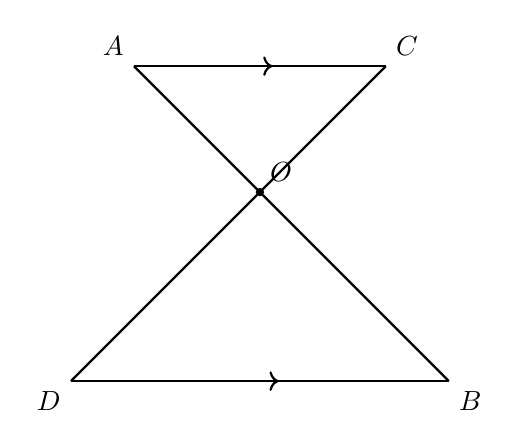
\begin{tikzpicture}[scale=1.0, thick]
  \coordinate (O) at (0, 0);
  \coordinate (A) at (-1.6, 1.6);
  \coordinate (B) at (2.4, -2.4);
  \coordinate (C) at (1.6, 1.6);
  \coordinate (D) at (-2.4, -2.4);

  \draw (A) -- (B);
  \draw (C) -- (D);
  \draw (A) -- (C);
  \draw (B) -- (D);

  % 平行箭头
  \draw[->] ($(A)!0.4!(C)$) -- ($(A)!0.55!(C)$);
  \draw[->] ($(D)!0.4!(B)$) -- ($(D)!0.55!(B)$);

  \node[above left]  at (A) {$A$};
  \node[below right] at (B) {$B$};
  \node[above right] at (C) {$C$};
  \node[below left]  at (D) {$D$};
  \node[above right] at (O) {$O$};
  \fill (O) circle (1.5pt);
\end{tikzpicture}
\end{document}
